\subsubsection{Mises à jour}
\begin{itemize}
    \item Réaliser une mise à jour depuis la branche stable si disponible
    \item Configurer le canal de mises à jour sur la dernière version stable (figure \ref{fig:04-configuration-updates-01})
    \item Maintenir actif le contrôle de mises à jour sur le dashboard (figure \ref{fig:04-configuration-updates-01})
\end{itemize}

\begin{tip}
    Ce dernier point peut être désactivé, notamment si le pare-feu n'aura pas accès à Internet.
\end{tip}

\begin{figure}[H]
    \centering
    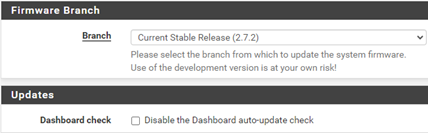
\includegraphics[width=0.7\textwidth]{04-Configuration/Images/04-configuration-updates-01.png}
    \caption{Configuration - Mises à jour}
    \label{fig:04-configuration-updates-01}
\end{figure}